\documentclass[border=6pt]{standalone}
\usepackage{tikz}
\usetikzlibrary{arrows.meta,positioning,calc,shapes.geometric,fit,backgrounds,patterns,matrix,decorations.pathreplacing}
\begin{document}
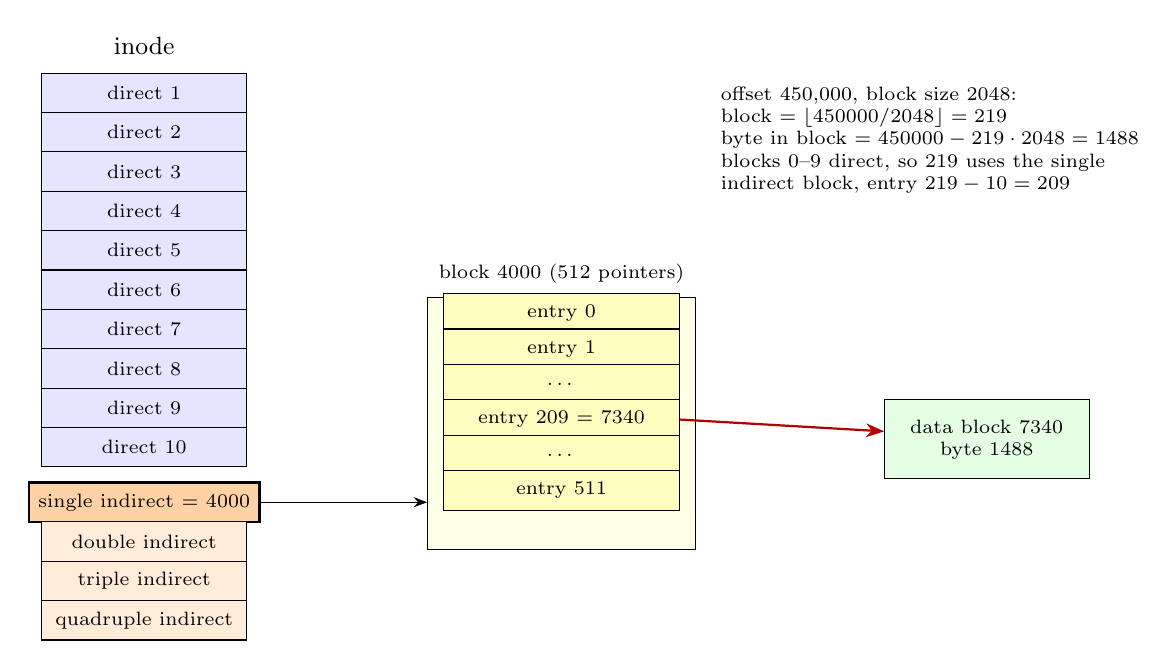
\begin{tikzpicture}[>=Stealth,font=\small]
\tikzstyle{c}=[draw,minimum height=0.5cm,minimum width=2.6cm,font=\scriptsize]
\node[font=\small] at (0,0.6) {inode};
\foreach \i in {1,...,10} \node[c,fill=blue!10] (d\i) at (0,-\i*0.5+0.5) {direct \i};
\node[c,fill=orange!35,line width=1pt] (s) at (0,-5.2) {single indirect = 4000};
\node[c,fill=orange!15] (d) at (0,-5.7) {double indirect};
\node[c,fill=orange!15] (t) at (0,-6.2) {triple indirect};
\node[c,fill=orange!15] (q) at (0,-6.7) {quadruple indirect};
\node[draw,minimum width=3.4cm,minimum height=3.2cm,fill=yellow!10] (ib) at (5.3,-4.2) {};
\node[font=\scriptsize] at (5.3,-2.3) {block 4000 (512 pointers)};
\foreach \k/\t in {0/{entry 0},1/{entry 1},2/{\ldots},3/{entry 209 = 7340},4/{\ldots},5/{entry 511}} \node[c,minimum width=3.0cm,fill=yellow!25] (e\k) at (5.3,-2.8-\k*0.45) {\t};
\draw[fill=green!10] (9.4,-4.9) rectangle node[font=\scriptsize,align=center]{data block 7340\\ byte 1488} (12.0,-3.9);
\draw[->] (s.east) -- (ib.west |- s.east);
\draw[->,thick,red!70!black] (e3.east) -- (9.4,-4.3);
\node[font=\scriptsize,align=left,anchor=west] at (7.2,-0.6) {offset 450,000, block size 2048:\\ block $=\lfloor450000/2048\rfloor=219$\\ byte in block $=450000-219\cdot2048=1488$\\ blocks 0--9 direct, so 219 uses the single\\ indirect block, entry $219-10=209$};
\end{tikzpicture}
\end{document}
